\documentclass[../EngineeringJournal_CDavis.tex]{subfiles}

\begin{document}

%%%%%%%%%%%%%%%%%%%%%%%%%%%%%%%%%%%%%%%%%%%%%%%%%%%%%
%%%%%%%%%%%%%%%%%%%%%%%%%%%%%%%%%%%%%%%%%%%%%%%%%%%%%

\chapter[Configuring Switch Security]{Configuring Switch\linebreak[1] 
Security Features\hspace*{\fill February 26, 2020}}
\noindent\textbf{{Packet Tracer Lab 10} \hspace*{\fill}{\textbf{CIT 167}}}\linebreak[1]
{{Spring 2020} \hspace*{\fill}{Chaz Davis}}                             
%===================================
%===================================


\hspace{0.2cm}
\begin{tcolorbox}[width=6.3in]
\scriptsize 
Sec features
  \begin{outline}
    \1  some thing
  \end{outline}
\end{tcolorbox}
\hspace{0.2cm}
\normalsize  
  

\clearpage

%===================================
\mysection{\textbf{Part 1: The Lab}}

\mysubsection{1}{Cable the Network}
I created and cabled the network according to the diagram.


\noindent\mysubsection{2}{Initialize and reload the router and switch}
I went into router configuration, and checked the flash.


\noindent\mysubsection{3}{Configure an IP address on PC-A}
I then went to PC-A and setup the IP configuration.

\noindent\mysubsection{4}{Configure basic settings on R1}
I went into R1 and entered the commands and then copied the running and
startup configs.


\noindent\mysubsection{5}{Configure basic settings on S1}
I ran the commands from the diagram, setting up basic settings and then
creatings and configuring vlan 99. 
\\When I issued the {\scriptsize{\verb$show vlan$}\normalsize} command 
it shows vlan 99 as active.
\\ When I ran the command {\scriptsize{\verb$show ip interface brief$}\normalsize} 
the status was ok and protocol was down. 
\\It shows as down becuase its not connected to a network.
\\After assigning f0/5 and f0/6 to vlan 99 no when running
the {\scriptsize{\verb$show ip int brief$}\normalsize} command
we can see vlan 99 as up.



\noindent\mysubsection{6}{Verify Connectivity between Devices}
\\As you can see in Fig.~\ref{Ping10} All of the pings were successful.



\begin{figure}[!hbt]\centering
\subfloat[PC-A pinging R1]{\label{Ping10a-r}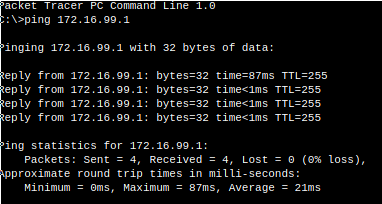
\includegraphics[width=.45\linewidth]{Figures/2020-02-26-032130_382x204_scrot.png}}\hfill
\subfloat[PC-A pinging S1]{\label{Ping10a-s}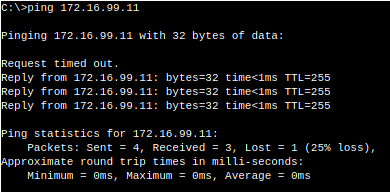
\includegraphics[width=.45\linewidth]{Figures/2020-02-26-032221_390x192_scrot.png}}\par 
\subfloat[S1 pinging R1]{\label{Ping10s-r}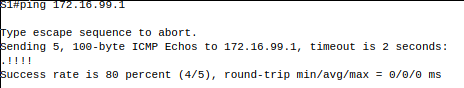
\includegraphics[width=.45\linewidth]{Figures/2020-02-26-032302_464x88_scrot.png}}
\caption{Successful pings on the network}
\label{Ping10}
\end{figure}

\clearpage

\noindent\mysubsection{7}{Configure SSH access on S1}
\\The ssh-version is 1.99
\\SSH will allow 3 retries
\\the default timeout is 120 secs


\noindent\mysubsection{8}{Modify the SSH configuration on S1}
\\It will now allow 2 retries, so a total of 3 attempts.
\\The timeout would be 75 seconds. So, 1 minute and 15 seconds.


\noindent{\bf{a)}}
It was successful, and the prompt said unauthorized access is strictly
prohibited, and the gave the S1 prompt with the octothorpe signifying the admin
account.


\noindent\mysubsection{9}{Configure general security features on S1}


\noindent{\bf{b)}}

\begin{figure}[!hbt]\centering
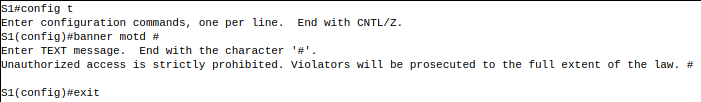
\includegraphics[width=.75\linewidth]{Figures/2020-02-26-035114_701x102_scrot.png}\par
\caption{Banner MOTD update}
\label{Banner10}
\end{figure}

\noindent{\bf{c)}}
The physical ports that are open are Fa0/5 and Fa0/6


\noindent{\bf{c \& d)}}
I ran the commands the output of 
{\scriptsize{\verb$show ip int brief$}\normalsize} gives us:


\begin{figure}[!hbt]\centering
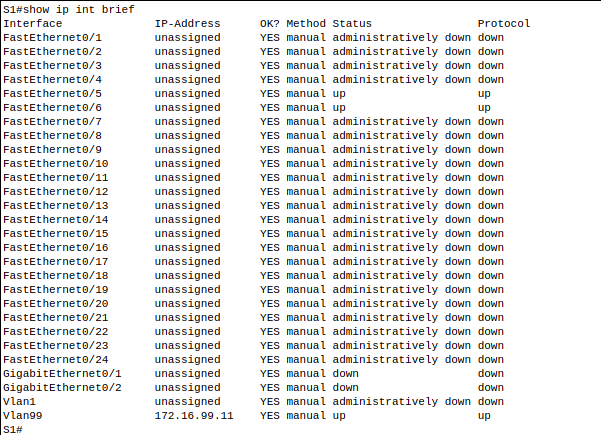
\includegraphics[width=.69\linewidth]{Figures/2020-02-26-040122_601x435_scrot.png}\par
\caption{Output of show ip int brief }
\label{Intbrief10}
\end{figure}

\clearpage

\noindent\mysubsection{10}{Configure and verify port security on S1}


\noindent{\bf{a)}}
The macaddress is 0004.9a08.6602


\noindent{\bf{b)}}
fa0/5 has a mac address of 0004.9a08.6602 and fa0/6 doesnt show on the table.


\noindent{\bf{c \& d)}}
The port status is {\scriptsize{\verb$Secure-Up$}\normalsize}.


\noindent{\bf{e)}}
From R1 I pinged PC-A as seen in Fig.~\ref{R1ping10}\subref{R1ping10A}.


\noindent{\bf{l)}}
The ping from R1 to PC-A was not successful. 


\noindent{\bf{m)}}
See Fig.~\ref{R1ping10}\subref{R1ping10B} for the output of
{\scriptsize{\verb$show int f0/5$}\normalsize}.


\noindent{\bf{p)}}
This time the ping was successful again. See
Fig.~\ref{R1ping10}\subref{R1ping10C}


\begin{figure}[!hbt]\centering
\subfloat[With a MAC-address]{\label{R1ping10A}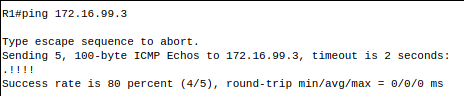
\includegraphics[width=.45\linewidth]{Figures/2020-02-26-041804_464x96_scrot.png}}\par
\subfloat[With no mac-address]{\label{R1ping10B}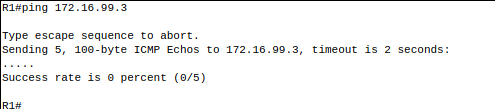
\includegraphics[width=.45\linewidth]{Figures/2020-02-26-042605_495x109_scrot.png}}\par 
\subfloat[With S1 back on]{\label{R1ping10C}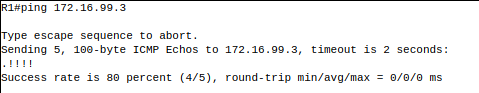
\includegraphics[width=.45\linewidth]{Figures/2020-02-26-043917_479x93_scrot.png}}\par 
\caption{Ping from R1 to PC-A}
\label{R1ping10}
\end{figure}



%===================================
\mysection{\textbf{Reflection}}

\mysubsection{1}{Why would you enable port security on a switch?}
To prevent unauthorized users to gain access to the LAN.


\noindent\mysubsection{2}{Why should unused ports on a switch be disabled?}
\\Any enabled port not in use could allow someone to come in and plug into
your network and gain access. So, it's best practice to disable any unused
ports.

%===================================

\end{document}
